\documentclass[tikz,border=2pt]{standalone}
\usepackage{amsmath,amssymb}
\usepackage{pgfplots}
\pgfplotsset{compat=1.18}
\usetikzlibrary{arrows.meta}
\begin{document}
% Graph of the Bertrand best-response correspondence BR_1(p_2): the open region p_1>p_2 for p_2<c,
% the ray [c,inf) at p_2=c, the empty set for c<p_2<=p^m, and the single point p^m for p_2>p^m.
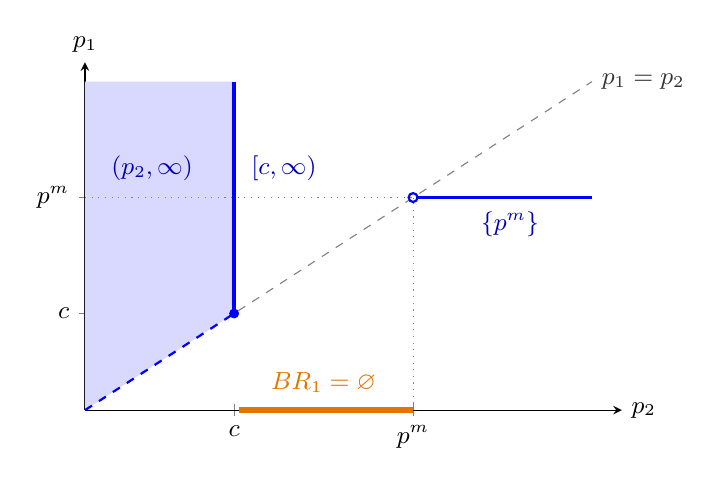
\begin{tikzpicture}[font=\small, >={Latex[length=2mm]}]
  \begin{axis}[
    axis lines=left,
    xmin=0, xmax=3.6, ymin=0, ymax=3.6,
    xtick={1,2.2}, xticklabels={$c$,$p^m$},
    ytick={1,2.2}, yticklabels={$c$,$p^m$},
    xlabel={$p_2$}, ylabel={$p_1$},
    xlabel style={at={(axis description cs:1,0)}, anchor=west},
    ylabel style={at={(axis description cs:0,1)}, anchor=south, rotate=-90},
    tick label style={font=\small},
    clip=false,
    width=8.4cm, height=6cm]
    % reference diagonal
    \draw[gray, thin, dashed] (axis cs:0,0) -- (axis cs:3.4,3.4);
    \node[gray!40!black, anchor=west] at (axis cs:3.4,3.4) {$p_1=p_2$};
    % p_2 < c : any price above p_2
    \fill[blue!15] (axis cs:0,0) -- (axis cs:1,1) -- (axis cs:1,3.4) -- (axis cs:0,3.4) -- cycle;
    \draw[blue, thick, dashed] (axis cs:0,0) -- (axis cs:1,1);
    \node[blue!70!black] at (axis cs:0.45,2.5) {$(p_2,\infty)$};
    % p_2 = c : the ray [c, inf)
    \draw[blue, very thick] (axis cs:1,1) -- (axis cs:1,3.4);
    \fill[blue] (axis cs:1,1) circle (1.8pt);
    \node[blue!70!black, anchor=west] at (axis cs:1.05,2.5) {$[c,\infty)$};
    % c < p_2 <= p^m : empty
    \draw[orange!90!black, line width=2pt] (axis cs:1.03,0) -- (axis cs:2.2,0);
    \node[orange!90!black, anchor=south] at (axis cs:1.6,0.08) {$BR_1=\varnothing$};
    % p_2 > p^m : {p^m}
    \draw[blue, very thick] (axis cs:2.2,2.2) -- (axis cs:3.4,2.2);
    \draw[blue, thick, fill=white] (axis cs:2.2,2.2) circle (1.6pt);
    \node[blue!70!black, anchor=north] at (axis cs:2.85,2.15) {$\{p^m\}$};
    \draw[gray, thin, dotted] (axis cs:2.2,0) -- (axis cs:2.2,2.2);
    \draw[gray, thin, dotted] (axis cs:0,2.2) -- (axis cs:2.2,2.2);
  \end{axis}
\end{tikzpicture}
\end{document}
